
%(BEGIN_QUESTION)
% Copyright 2006, Tony R. Kuphaldt, released under the Creative Commons Attribution License (v 1.0)
% This means you may do almost anything with this work of mine, so long as you give me proper credit

Suppose a gas-fired water heater is controlled manually, with a human operator observing a temperature indicator on the hot water outlet pipe and actuating a fuel gas control valve:
  
$$\includegraphics[width=15.5cm]{i01452x01.eps}$$

Does the operator play the part of a {\it direct-acting} controller, or a {\it reverse-acting} controller, in this process control scenario?

Also, identify the {\it process variable}, {\it setpoint}, and {\it manipulated variable} in this manual control system.

\underbar{file i01452}
%(END_QUESTION)





%(BEGIN_ANSWER)

The human operator plays the part of a {\it reverse-acting} controller, because the valve action must be opposite of any changes in process variable.  For example, if the water temperature increases, then the operator should move the control valve further closed.

\begin{itemize}
\item{} PV = water temperature
\item{} SP = ideal (target) water temperature, in operator's mind
\item{} MV = Fuel gas control valve position
\end{itemize}

%(END_ANSWER)





%(BEGIN_NOTES)


%INDEX% Basics, control: direct versus reverse controller action

%(END_NOTES)


